% DESCRIPTION OF THE DATA
In the years 2009-2012 and 2014 the compressive strength of clay block masonry was measured for a variable number of specimens in a series of compression tests.
In addition, the compressive strengths of bricks and mortar were recorded for realizations from the same ensembles that were later used for the construction of the masonry wall.
The tests were performed at the laboratories of the Department of Civil, Environmental and Geomatic Engineering of ETH Z\"{u}rich.
Two photographs that were made during the tests are shown in \cref{fig:ICASP:Testing}.
In \cref{tab:ICASP:Data} the experimental data are summarized.
% DATA SCARCITY
Five batches of experiments were performed in total.
At the system- and the component level the available data is generally scarce.
Especially in the years 2011 and 2012 the number of component-level tests was very limited.
Moreover, in the years 2009 and 2010 brick units from the same ensemble were used.
% FIGURES: TESTING
\begin{figure}[htbp]
  \centering
  \begin{subfigure}[b]{0.49\textwidth}
    \centering
    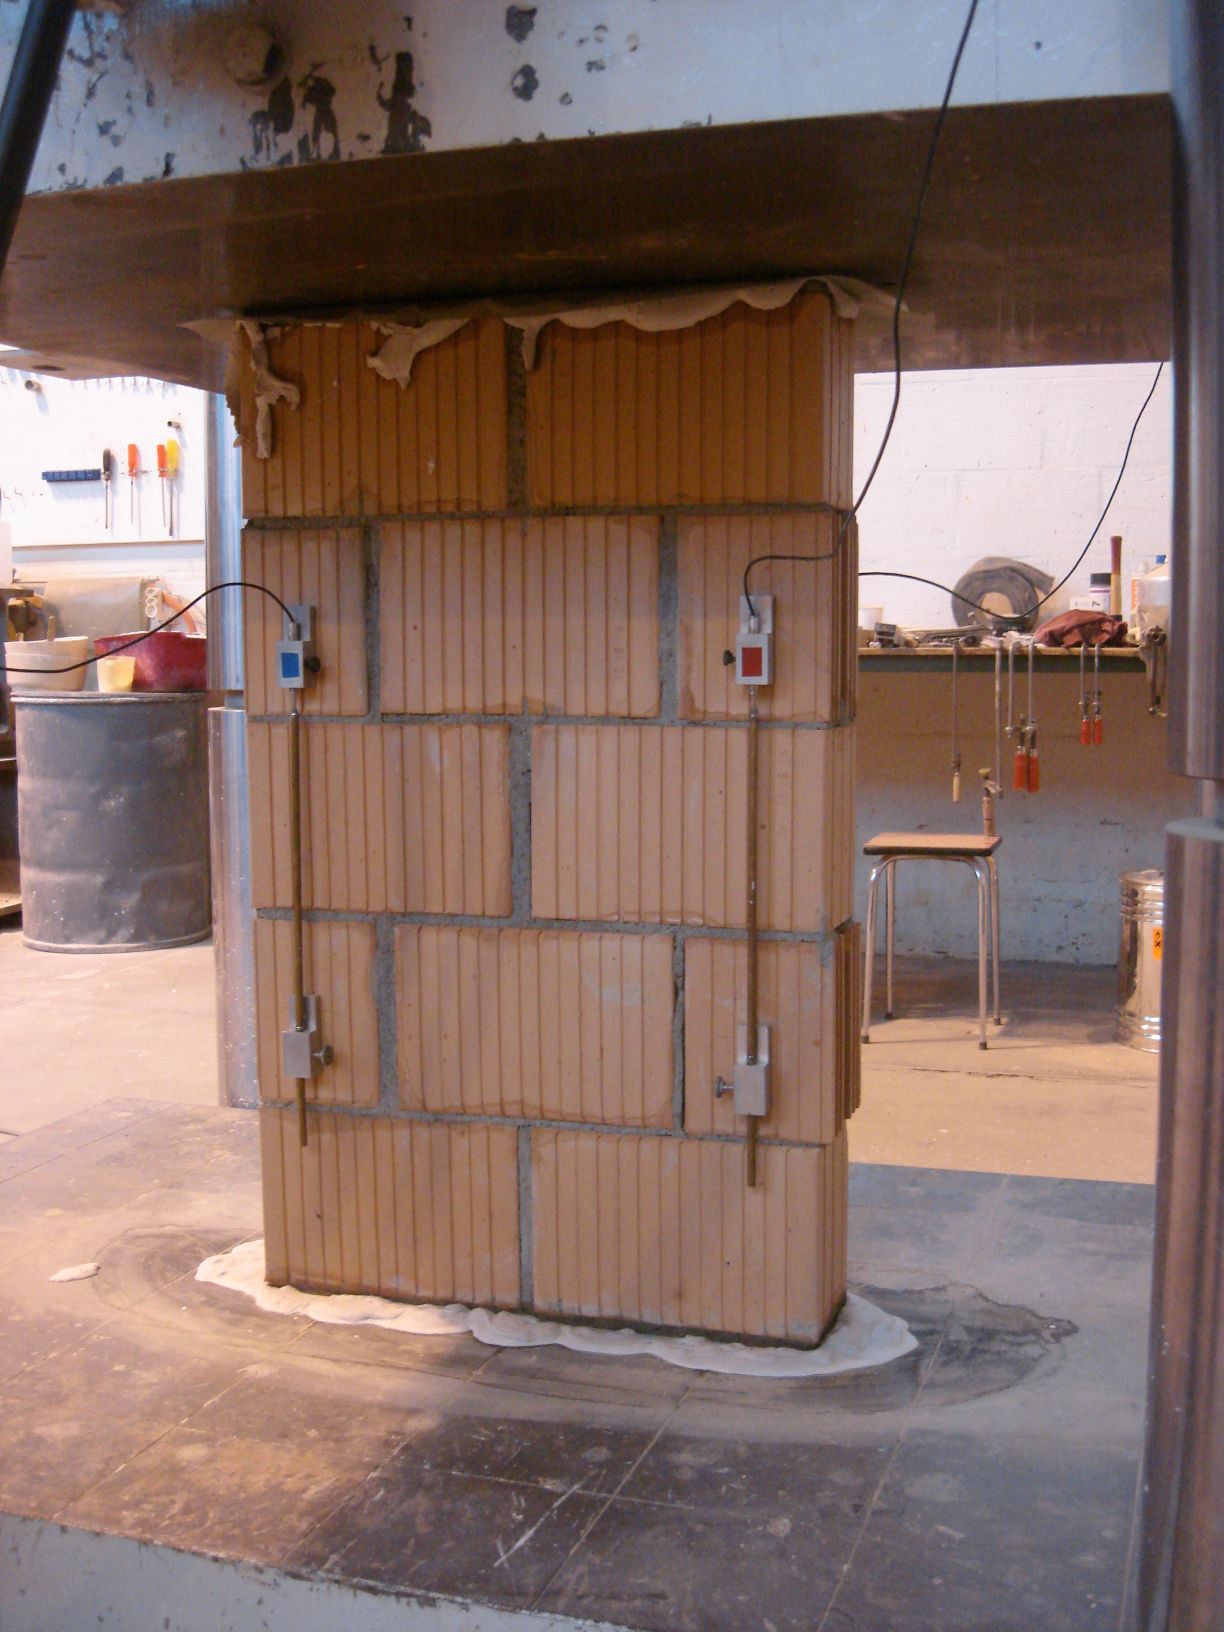
\includegraphics[height=\ICASPphotoHeight]{fig_ICASP_Test1}
    \caption[Before failure]{Before failure.}
    \label{fig:ICASP:Testing:1}
  \end{subfigure}\hfill%
  \begin{subfigure}[b]{0.49\textwidth}
    \centering
    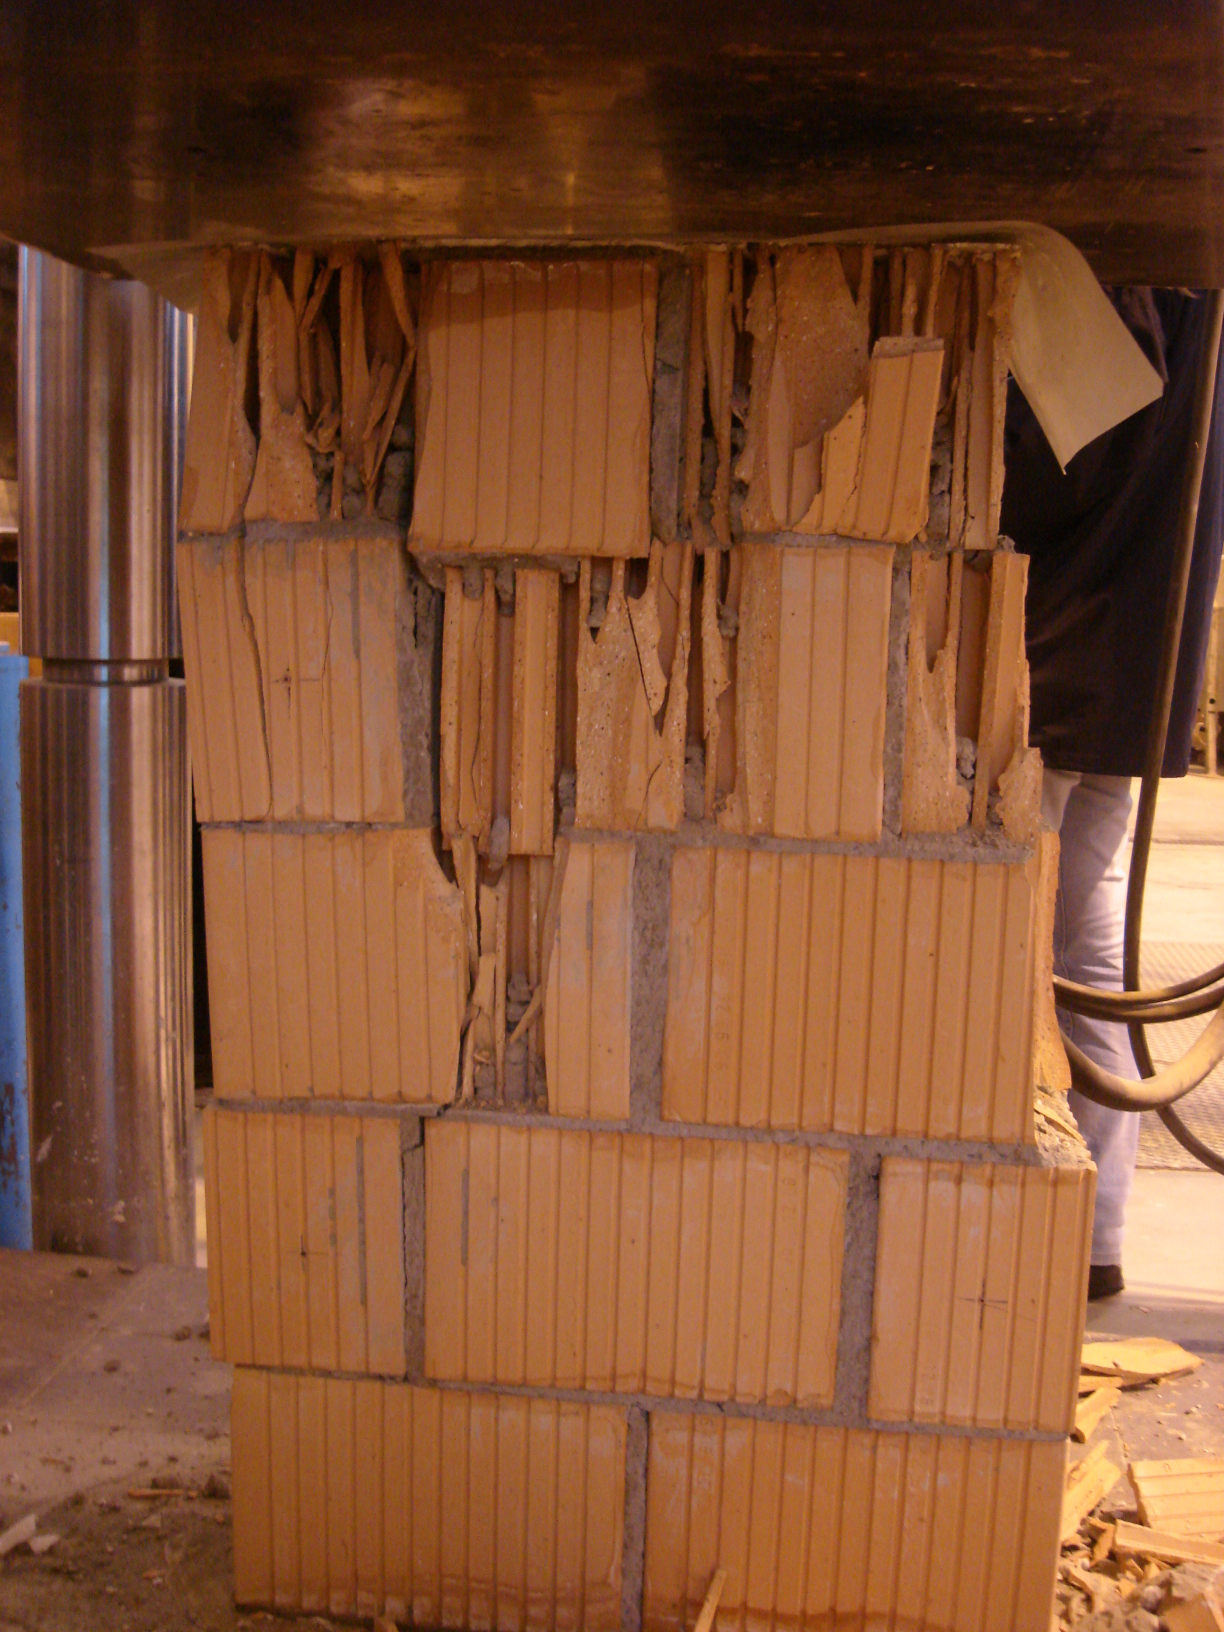
\includegraphics[height=\ICASPphotoHeight]{fig_ICASP_Test2}
    \caption[After failure]{After failure.}
    \label{fig:ICASP:Testing:2}
  \end{subfigure}%
  \caption[Compression test]{Compression test.
          A specimen is shown before its failure in \subref{fig:ICASP:Testing:1} and thereafter in \subref{fig:ICASP:Testing:2}.
          }
  \label{fig:ICASP:Testing}
\end{figure}
% TABLE: EXPERIMENTAL DATA
\begin{table}[htbp]
  \caption[Experimental data]{Experimental data.
           Data are shown for tests of clay block masonry that were performed in the years 2009-2012 and in 2014.
           Blocks from the same ensemble were used in 2009 and 2010.
           Thus the corresponding rows show duplicate data entries.
          }
  \label{tab:ICASP:Data}
  \centering
  \resizebox{\linewidth}{!}{
  \begin{tabular}{lr|ccccccccccccc}
    \toprule
    \multicolumn{2}{r|}{2009} & \multicolumn{13}{l}{Batch 1} \\
    \midrule
    \(f_w\) & \multirow{3}{*}{\rotatebox[origin=c]{90}{\([\unit[]{MPa}]\)}}
    & \(9.41\)  & \(5.53\)  & \(7.98\)  & \(8.86\)  & \(6.67\)  & \(7.17\)  & \(7.92\)  & -         & -         & -         & -        & -        & -        \\
    \(f_b\) &
    & \(33.58\) & \(34.55\) & \(37.1\)  & \(39.21\) & \(39.63\) & \(36.1\)  & \(35.46\) & \(37.61\) & \(35.6\)  & \(36.26\) & \(35.2\) & \(32.7\) & \(36.6\) \\
    \(f_m\) &
    & \(15.8\)  & \(16.1\)  & \(14.4\)  & \(14.8\)  & \(16.1\)  & \(15.4\)  & \(13.9\)  & \(14.6\)  & \(14.6\)  & \(14.4\)  & \(16.8\) & \(16.1\) & -        \\
    \midrule
    \multicolumn{2}{r|}{2010} & \multicolumn{13}{l}{Batch 2} \\
    \midrule
    \(f_w\) & \multirow{3}{*}{\rotatebox[origin=c]{90}{\([\unit[]{MPa}]\)}}
    & \(6.67\)  & \(6.12\)  & \(5.91\)  & \(8.3\)   & \(6.44\)  & \(5.32\)  & \(6.7\)   & -         & -         & -         & -        & -        & -        \\
    \(f_b\) &
    & \(33.58\) & \(34.55\) & \(37.1\)  & \(39.21\) & \(39.63\) & \(36.1\)  & \(35.46\) & \(37.61\) & \(35.6\)  & \(36.26\) & \(35.2\) & \(32.7\) & \(36.6\) \\
    \(f_m\) &
    & \(12.5\)  & \(12.94\) & \(12.43\) & \(13.33\) & \(12\)    & \(12.32\) & -         & -         & -         & -         & -        & -        & -        \\
    \midrule
    \multicolumn{2}{r|}{2011} & \multicolumn{13}{l}{Batch 3} \\
    \midrule
    \(f_w\) & \multirow{3}{*}{\rotatebox[origin=c]{90}{\([\unit[]{MPa}]\)}}
    & \(4.32\)  & \(3.71\)  & \(6.06\)  & \(4.95\)  & \(4.29\)  & \(2.8\)   & \(6.28\)  & \(4.22\)  & \(5.23\)  & -         & -        & -        & -        \\
    \(f_b\) &
    & \(23.8\)  & \(26.8\)  & \(25.7\)  & -         & -         & -         & -         & -         & -         & -         & -        & -        & -        \\
    \(f_m\) &
    & \(14.9\)  & \(14.7\)  & \(14.9\)  & \(15.4\)  & \(14.7\)  & \(14.6\)  & -         & -         & -         & -         & -        & -        & -        \\
    \midrule
    \multicolumn{2}{r|}{2012} & \multicolumn{13}{l}{Batch 4} \\
    \midrule
    \(f_w\) & \multirow{3}{*}{\rotatebox[origin=c]{90}{\([\unit[]{MPa}]\)}}
    & \(8\)     & \(7.87\)  & \(8.1\)   & \(7.53\)  & \(8.14\)  & \(6.99\)  & \(7.82\)  & \(9.13\)  & \(5.87\)  & \(7.71\)  & -        & -        & -        \\
    \(f_b\) &
    & \(37\)    & \(39.9\)  & \(38\)    & -         & -         & -         & -         & -         & -         & -         & -        & -        & -        \\
    \(f_m\) &
    & \(26.9\)  & \(28.1\)  & \(17\)    & \(16.2\)  & \(18.7\)  & \(21.1\)  & -         & -         & -         & -         & -        & -        & -        \\
    \midrule
    \multicolumn{2}{r|}{2014} & \multicolumn{13}{l}{Batch 5} \\
    \midrule
    \(f_w\) & \multirow{3}{*}{\rotatebox[origin=c]{90}{\([\unit[]{MPa}]\)}}
    & \(6.53\)  & \(7.01\)  & \(6.12\)  & \(5.94\)  & \(7.14\)  & \(5.69\)  & \(5.82\)  & \(6.34\)  & \(5.96\)  & -         & -       & -         & -        \\
    \(f_b\) &
    & \(28.15\) & \(27.74\) & \(28.05\) & \(27.20\) & \(26.25\) & \(23.15\) & \(26.69\) & \(28.04\) & \(27.69\) & \(26.73\) & -       & -         & -        \\
    \(f_m\) &
    & \(11.73\) & \(12.19\) & \(12.13\) & \(10.49\) & \(10.34\) & \(10.44\) & -         & -         & -         & -         & -       & -         & -        \\
    \bottomrule
  \end{tabular}
  }
\end{table}
\par % MEASUREMENTS VS. PREDICTIONS
We observe that the empirical relation \cref{eq:ICASP:EmpiricalRelation} generally overpredicts the masonry wall compressive strength.
In \cref{fig:ICASP:MeasVsPred:2009} the actually acquired data for \(i=1\), i.e.\ for the year 2009, is shown together with the correspondingly predicted characteristic value.
% COEFFICIENTS
The values \(k^\prime = 0.45\), \(\alpha^\prime = 0.7\), \(\beta^\prime = 0.3\) provided in \cite{Standard:Eurocode6:1-1} were used.
Brick unit data \(\tuple{f_{b,ik}}\) have been normalized according to their geometry.
% IDENTIFICATION/TRANSFORMATION
Moreover a lognormal distribution of the form \cref{eq:ICASP:ProbabilisticInterpretation} is shown,
where \(\alpha=\alpha^\prime\) and \(\beta=\beta^\prime\) have been identified with the corresponding coefficients from \cite{Standard:Eurocode6:1-1}.
The remaining coefficient \(k = k^\prime \cdot \exp (1.645 \sqrt{\alpha_i^2 \sigma_{b,i}^2 + \beta_i^2 \sigma_{m,i}^2} + \alpha_i [\sigma_{b,i}^2 / 2] + \beta_i [\sigma_{m,i}^2 / 2])\)
has been set in order that the \(\unit[5]{\%}\)-quantile equals \cref{eq:ICASP:EmpiricalRelation}.
Note that the abovementioned identification/transformation of the coefficients establishes another way of extending \cref{eq:ICASP:EmpiricalRelation} and comparing it to \cref{eq:ICASP:ProbabilisticInterpretation}.
In this paper we do not pursue this approach, though.
% FIGURE: MEASUREMENTS VS. PREDICTIONS
\begin{figure}[ht]
  \centering
  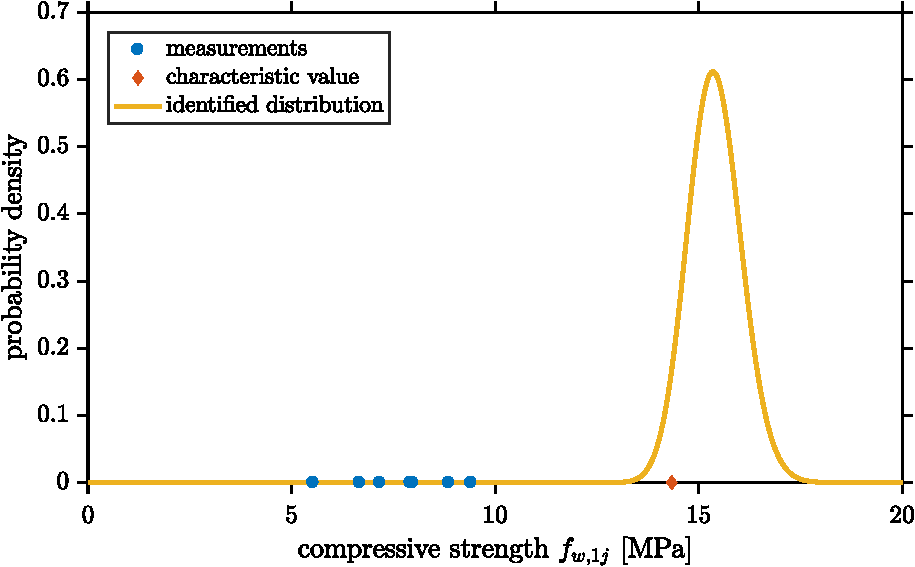
\includegraphics[width=\ICASPfigWidth]{fig_ICASP_PredVsMeas_2009}
  \caption[Data and predictions for 2009]{Data and predictions for 2009.
           The data, its expected \(\unit[5]{\%}\)-quantile and a corresponding lognormal distribution are shown.
           The data are overpredicted.
          }
  \label{fig:ICASP:MeasVsPred:2009}
\end{figure}
\par % QUESTIONS
Of course, the unexpected code/measurement discrepancy raises important questions.
Anticipating our results it is said that we will not be able to satisfactorily explain this discrepancy.
Instead we will calibrate the coefficients \(k\) and \(\alpha\) in a way that leads to better predictions.
Those predictions are valid for the testing machine and the materials used in our laboratory.
Using the predictions outside their scope of applicability is questionable and should only be done with utmost caution.